\documentclass[conference]{IEEEtran}


  	\usepackage[pdftex]{graphicx}
  	\graphicspath{{../pdf/}{../jpeg/}}
	\DeclareGraphicsExtensions{.pdf,.jpeg,.png}

	\usepackage[cmex10]{amsmath}
	\usepackage{mathabx}
	\usepackage{algorithmic}
	\usepackage{array}
	\usepackage{mdwmath}
	\usepackage{mdwtab}
	\usepackage{eqparbox}
	\usepackage{url}
 \usepackage{multirow}
 \usepackage{verbatim}
	\hyphenation{op-tical net-works semi-conduc-tor}
\usepackage{hyperref}
\hypersetup{
    colorlinks=true,
    linkcolor=blue,
    filecolor=magenta,      
    urlcolor=cyan,
    pdftitle={Overleaf Example},
    pdfpagemode=FullScreen,
    }

\urlstyle{same}

\begin{document}

\title{\LARGE Online Hotel Booking Recommendation System}

% \author{\authorblockN{Leave Author List blank for your IMS2013 Summary (initial) submission.\\ IMS2013 will be rigorously enforcing the new double-blind reviewing requirements.}
% \authorblockA{\authorrefmark{1}Leave Affiliation List blank for your Summary (initial) submission}}

 \author{\authorblockN{Nikhil Dutt (A14285637) \authorrefmark{2}, Abhishek Khare (A59010306) \authorrefmark{2} }
}

\maketitle

\begin{abstract}
Planning a vacation or weekend escape can be an overwhelming affair because with thousands of hotels to choose from it’s difficult to know which one would suit your personal preferences. So in order to simplify this process we plan to create a recommendation strategy for hotel booking. We would use data analysis techniques for pre-processing/standardizing the data, and make inferences based on the statistical analysis of the data. We would use various statistical classification strategies and then perform hypothesis testing and then make conclusions based on it.
\\
\\ Project Type: Data Exploration and Inference.
\\
\end{abstract}

\IEEEoverridecommandlockouts
\begin{keywords}
Logistic Regression, Bayesian Decision Rule, Support Vector Machines (SVM), Decision Tree
\end{keywords}

\IEEEpeerreviewmaketitle


% ===================
% # I. Introduction #
% ===================

\section{\textbf{Introduction}}
The Expedia Group wants to eliminate any inconveniences and difficulties from their hotel search process by providing personalized hotel recommendations to their users. Given that this site sees hundreds of millions of visitors every month, this task involves a lot of complexities.
\subsection{Problem Statement:}
Designing a fairly reliable and accurate recommendation system for online hotel booking based on data analysis and statistical machine-learning techniques applied to the existing dataset. 
\subsection{Problem Description:}
Currently, Expedia makes use of search parameters to adjust their hotel recommendations, but there isn't enough customer-specific data to personalize them for each user. In this task, we aim to contextualize the customer data and predict which hotel group (out of 100 different hotel groups) a user will be most likely to stay at. To do this, we will use different techniques including Logistic Regression, Bayesian Decision Rule, Support Vector Machines, Decision Trees and compare the results of each to determine the most successful approach. Along with this, we will identify the key drivers or features that lead to successful recommendations.
\subsection{Project's Significance:}
This problem is significant as every company aims to maximize its profitability and to do that they must ensure that they retain customers by providing them with high-quality services. Insights from customer-specific data as well as a recommendation system can allow the business to generate more accurate recommendations and attract more users.  
\subsection{Target Questions and Inferences:}
Our goal is to find answers to questions like - What are the user preferences when booking a hotel? Do users books a hotel as a part of a package deal? Do mobile users make a booking more frequently than other users? Which month/season gets more online bookings? What is the statistical distribution of the users' duration of stay? etc. 
% =======================================================
% # II. Impact of traps on large signal characteristics #
% =======================================================

\section{\textbf{Description of Dataset}}
For this project, we have used a publicly available dataset from Kaggle which includes logs of Expedia's customer behaviour. This data is separated into two different sets: the test data (used only for evaluating performance of our models) and the training set (which will be used for data exploration and training our models). These two sets are split based on time: training data are from 2013 and 2014, while test data are from 2015. Upon further inspection of the data we see that we are provided with 24 different features. Our target variable (the one we are trying to predict) is ‘hotel-cluster’ and we will essentially use the other 23 variables (depending on which ones we deem useful) to make a prediction for a hotel cluster. These hotel clusters serve as good identifiers to which types of hotels people are going to book, while avoiding outliers such as new hotels that don't have historical data. 


% =============================================
% # III. Modeling and consistency validations #
% =============================================

\section{\textbf{Data Exploration}}

In our training data, we have 200,000 rows (customer logs) and 24 columns. After performing some basic data cleaning, we find that three features have missing data: distance from origin to destination, check-in date and check-out date. Since check-in and check-out date account for less than 1\% of the missing data, it would make more sense to drop these records since it would be extremely difficult to impute these. Distance from origin to destination accounts for 34\% of the missing data so we must implement a data imputation strategy for these records. We simply replace missing values in this field with the mean distance from origin to destination of the entire training set. After these changes, we are now working with a training set that has 199,823 instances.

\textbf{Correlation Analysis:} For this type of analysis we will be using the concept of correlation from class. We will be using the Pearson coefficient to determine the degree to which each feature is correlated with each other. When the coefficient is closer to +1, 0, and -1, we have that the pair of features is strongly positively correlated, uncorrelated and strongly anti-correlated respectively. The following formula was used to calculate the Pearson coefficient:
\begin{figure}[ht!] %!t
\centering
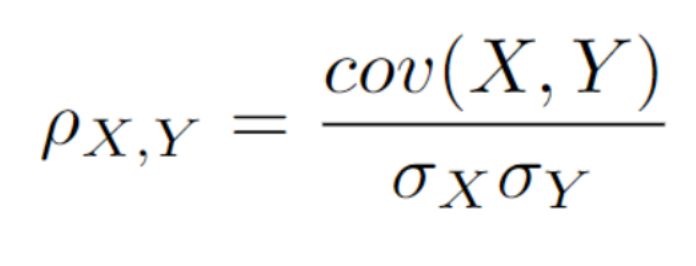
\includegraphics[width=1.5in]{pearson.PNG}
\label{pearson}
\end{figure}

Figure 1 shows a heatmap containing the correlation coefficients between various features of the training set. Darker colors denote low correlation and brighter colors denote higher correlation. Nothing interesting really stands out here as most features do not seem to be correlated with hotel cluster and the features don't seem to be correlated among themselves. Ideally if we saw that certain features were highly correlated with each other, we would remove one of them since we would not want the effect of that particular variable to appear twice in the model. Since we see that none of the attributes correlate very well with each other, we can proceed by using all the attributes in the dataset.

\begin{figure}[ht!] %!t
\centering
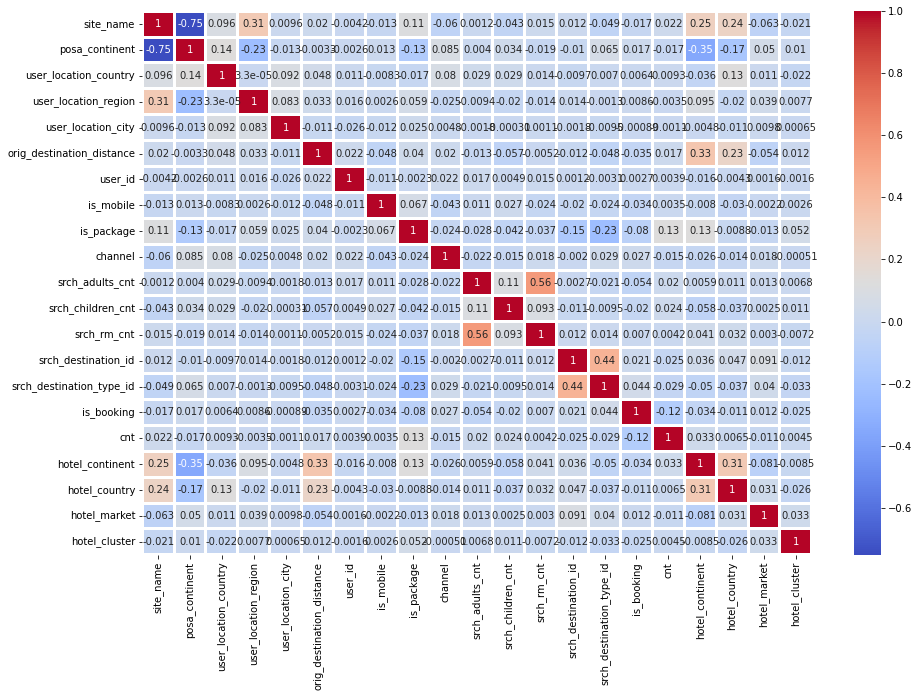
\includegraphics[width=3.5in]{heatmap.png}
\caption{Correlation among all features in the dataset}
\label{heatmap}
\end{figure}
While conducting basic exploratory data analysis, we observed that overall the number of bookings through mobile phones is less compared to bookings through the Expedia website as seen in Figure 2. This information could be used to suggest that Expedia make a more interactive and easy to use website so that users can book their hotels with greater ease. Additionally, we see that most bookings made were not part of a travel package (less than half of the bookings were through a package).

There are 6 different continents in this dataset as seen in the figure. 'posa\_continent' refers to the continent from where a specific booking was made while hotel\_continent refers to the continent where the booking was for. We can see that majority of bookings are made from the site in Continent 3. There could be a variety of reasons for this such as people there having more expending power. Expedia could possibly increase its business by increasing more hotel options, more variety, better user experience, etc. For other continents Expedia can lower its prices on hotels and provide discounts or loyalty points. The figure also tells us that while most bookings are made from Continent 3, the majority of the booking destinations are in Continent 2. That is, most people are from Continent 3 and travel to Continent 2. In figure X we see data for each month across three years and that the highest number of bookings was consistently in the month of August. It is likely the case that most users book in this period as it is the peak of the summer holidays.

In our analysis it was clear that 2014 had the most number of bookings. If we take a look at figure X which shows month wise bookings, the graph peaks at certain months in 2014 and clearly exceeds bookings made in 2013. We then see that the number of bookings in 2015 decreases heavily. Therefore, it might be a good idea for Expedia to compare what was the strategy in 2014 versus 2015 which caused such a considerable decline in the number of bookings.

% ==================
% # IV. CONCLUSION #
% ==================

\section{\textbf{Binary and Multi-Class Supervised Classification Techniques:}}
For the classification problem, we need to basically make two types of classifications and answer/predict the following two unknowns.
\begin{itemize}
\item Whether the given user would make a booking ? - This involves Binary Classification as we have a yes/no answer.
\item User hotel cluster preference - This involves Multi-Class classification as we need to predict which cluster of the hotels would the user prefer. The given Expedia dataset contains 100 hotel clusters and the classifier has to predict which of those hotel cluster has the better chances of getting picked by the user and would thus be recommended to the user.
\end{itemize}

\subsection{Classification Methods:}

\subsubsection{Naive Bayes Decision Classifier}
Naive Bayes Classifiers and basic probabilistic Machine learning Classifiers based on Bayes Decision Rule. \cite{stat_learning} \\
Naive Bayes Classifiers takes the training input vectors and considers each of its input feature to be independent of one other, and maps them on the feature vector space independently and creates a statistical probability distribution of the training vectors based on the classes they belong to. For predicting the class of the test vector it calculates the Maximum a posteriori (MAP) probability and calculates the probability of that test vector belonging to each class based on the Bayes Theorem. The Predicted class would be the one that had the highest probability value. 
\begin{figure}[htbp] %!t
\centering
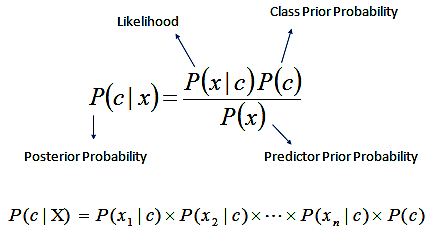
\includegraphics[width=2.5in]{naive_bayes_icon.PNG}
\label{Naive Bayes classification mechanism}
\caption{Naive Bayes Classifier - computing posterior probability}
\end{figure}

\subsubsection{Support Vector Machines (SVM)}
Support Vector Machines (SVM) is a machine learning algorithm for the statistical classification of input data making a prediction of its desired class based on the input vector.\cite{svm} \\
SVM Working Mechanism for binary classification - The SVM Algorithm takes in the input vector from the training dataset and maps it in its respective vector space one at a time. It maps all the training vectors into the vector space and it does so while creating a decision boundary such as the cumulative distance between the vectors belonging to the two classes is maximized. i.e, the decision boundary should separate the two types of input vectors in the best possible (optimal) way such that the vectors could be differentiated with a high margin of the distance between them.
\begin{figure}[htbp] %!t
\centering
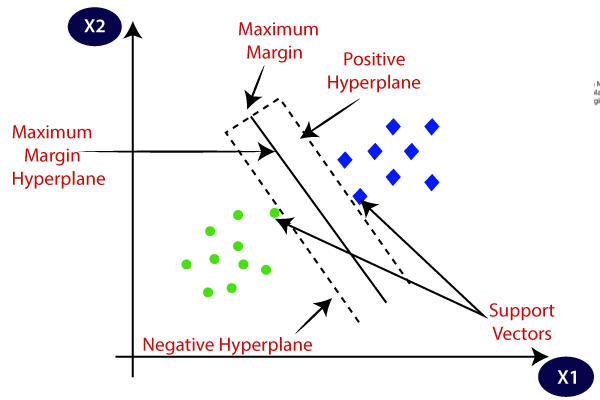
\includegraphics[width=2.5in]{svm_image.PNG}
\label{SVM classification mechanism}
\caption{SVM classification mechanism}
\end{figure}

This Mechanism can be optimized in various ways by changing the decision boundary's shape - like using linear, polynomial or rbf kernel. The algorithm can also be optimized by tweaking the parameters of the decision boundary, etc. \\
This method of binary classification SVM can further be extended to solve the Multi-Class classification problem. In this project we have used SVM with 'Linear' and 'RBF' (Radial Basis Function) Kernel. \\
\subsubsection{Decision Tree Classification}
Decision Tree Learning is a supervised, statistical machine-learning algorithm that makes predictions based on a classification tree formed using the input training data. This technique of learning can also be used in performing regression.\\
\begin{figure}[htbp] %!t
\centering
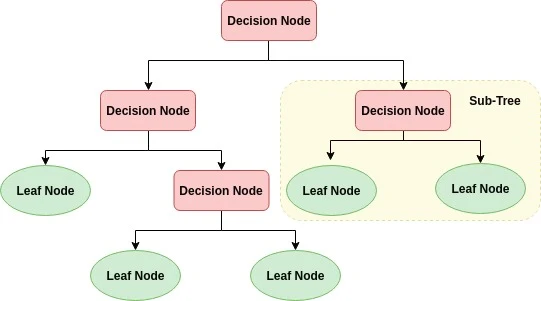
\includegraphics[width=2.5in]{decision_tree.PNG}
\label{Decision Tree Classification}
\caption{Decision Tree Classification}
\end{figure}
The accuracy of this technique could further be improved using ensemble methods such as - boosted trees where we incrementally build an ensemble by training every new instance to fix previously mislabelled vectors. \cite{stat_learning} \cite{d_tree}

\section{\textbf{Hotel Cluster Classification:}}
In order to classify which cluster of hotels would be the user's choice we would use various machine learning methods and would train these ML classifiers on the dataset. For this project, we have tried classification methods like - Support Vector Machines, Naive Bayes Decision Classifier, and Decision Tree Classifier. \\
We standardized the input training vector data and then applied these methods and set the hyperparameters based on the standard hyperparametric optimization techniques.\cite{9257290}

\begin{table}[htbp]
\begin{tabular}{|c|c|}
\hline
\textbf{Classification Technique} & \textbf{Cluster Classification Accuracy} \\ \hline
SVM (Linear Kernel)               & 52.4 \%                                  \\ \hline
SVM (RBF Kernel)                  & 61.2 \%                                  \\ \hline
Naive Bayes Decision Rule         & 59.2 \%                                  \\ \hline
Decision Tree                     & 68.5 \%                                    \\ \hline
\end{tabular}
\caption{Hotel Cluster Classification Accuracy Values}
\end{table}
By observing these classification accuracy values, we can deduce that although the above mentioned classification techniques might not be on par with the industry standards (which involve computationally expensive and memory intensive neural network architectures) but can be used as a fairly decent benchmark for an above average recommendation system.
\section{\textbf{User Decision Prediction}}
In this part of the project we would like to formulate a technique to determine Whether a user would make a booking or not.\\
This is a binary classification problem and we would use supervised machine-learning classification methods for predicting if a user will make an online booking.
\begin{table}[htbp]
\begin{tabular}{|c|c|}
\hline
\textbf{Classification Technique} & \textbf{Binary Classification Accuracy} \\ \hline
SVM (Linear Kernel)               & 83.3 \%                          \\ \hline
SVM (RBF Kernel)                  & 90.2 \%                          \\ \hline
Naive Bayes Decision Rule         & 91.9 \%                          \\ \hline
Decision Tree                     & 92.4 \%                          \\ \hline
\end{tabular}
\caption{Binary Classification Accuracy Values}
\end{table}
We observe such high accuracy values in predicting the 'is\_booking' parameter as compared to cluster classification accuracy values because in our input distribution we have a very skewed distribution of 'is\_booking' label (as majority of the users don't make a booking when they perform a hotel search online). Hence the classifiers predict 0 in most of the cases (0 here means no booking was made).\\
We can observe this better using Confusion Matrix for the respective methods (Table III) 

\begin{table}[htbp]
\begin{tabular}{|cc|cc|}
\hline
\multicolumn{2}{|c|}{\multirow{2}{*}{\textbf{\begin{tabular}[c]{@{}c@{}}Confusion \\ Matrix\end{tabular}}}} & \multicolumn{2}{c|}{\textbf{Predicted Class}}                        \\ \cline{3-4} 
\multicolumn{2}{|c|}{}                                                                                      & \multicolumn{1}{c|}{\textbf{0 (No Booking)}} & \textbf{1 (Booking )} \\ \hline
\multicolumn{1}{|c|}{\multirow{2}{*}{\textbf{Test Class}}}             & \textbf{0 (No Booking)}            & \multicolumn{1}{c|}{95.9 \%}                 & 4.1 \%                \\ \cline{2-4} 
\multicolumn{1}{|c|}{}                                                 & \textbf{1 (Booking)}               & \multicolumn{1}{c|}{39.3 \%}                 & 61.7 \%               \\ \hline
\end{tabular}
\caption{Confusion Matrix for Binary Decision Tree Classifier}
\end{table}
Similarly, we can also observe the confusion matrix for Naive Bayes Classifier and observe that the amount of false-positive cases remains relatively unchanged but the proportion of false-negative classifications increase, thus reducing the overall accuracy slightly.

\begin{table}[htbp]
\begin{tabular}{|cc|cc|}
\hline
\multicolumn{2}{|c|}{\multirow{2}{*}{\textbf{\begin{tabular}[c]{@{}c@{}}Confusion \\ Matrix\end{tabular}}}} & \multicolumn{2}{c|}{\textbf{Predicted Class}}                        \\ \cline{3-4} 
\multicolumn{2}{|c|}{}                                                                                      & \multicolumn{1}{c|}{\textbf{0 (No Booking)}} & \textbf{1 (Booking )} \\ \hline
\multicolumn{1}{|c|}{\multirow{2}{*}{\textbf{Test Class}}}             & \textbf{0 (No Booking)}            & \multicolumn{1}{c|}{96.0 \%}                 & 4.0 \%                \\ \cline{2-4} 
\multicolumn{1}{|c|}{}                                                 & \textbf{1 (Booking)}               & \multicolumn{1}{c|}{44.9 \%}                 & 55.1 \%               \\ \hline
\end{tabular}
\caption{Confusion Matrix for Naive Bayesian Classifier}
\end{table}

\begin{comment}
\section{\textbf{Predictive Task}}
\textbf{Logistic Regression (LR)}: Logistic Regression is similar to linear regression except that logistic regression predicts if something is true or false rather than predicting something continuous. Additionally instead of fitting a line to the data, logistic regression fits an ‘S-shaped’ logistic function and hence is primarily used for classification. LR models the chance of an outcome based on individual characteristics. Since chance is a ratio what actually gets modeled is the logarithm of chance given by:
\begin{figure}[ht!] %!t
\centering
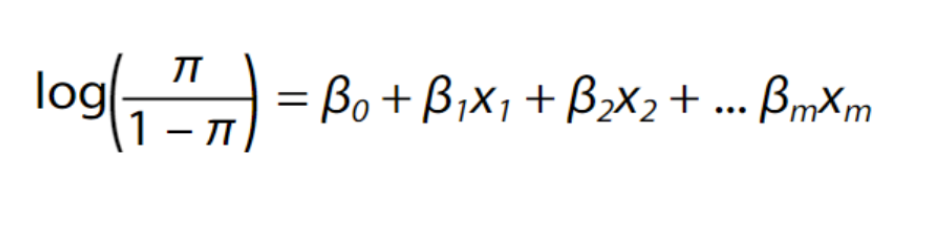
\includegraphics[width=3in]{LR.PNG}
\label{pearsona}
\end{figure}

where $\pi$ is probability of an event (e.g. belonging to a hotel cluster in our case), \(\beta_i\) are the regression coefficients and \(x_i\) are the predictive variables or features. 



% ==================
% # ACKNOLEDGMENTS #
% ==================

% use section* for acknowledgement
%\section*{Acknowledgment}
% The authors would like to thank...


% ==============
% # REFERENCES #
% ==============
\end{comment}

\section{\textbf{Results and Observations}}
Based on our analysis of the output, we can observe the following aspects of this data.
\begin{itemize}
\item Many of features in the input data are weakly correlated (as shown in Fig 1). hence, many of the input features can be considered as almost independent when modeling the data.
\item We observe the user's behavior (choices) and how it varies to some degree based on region and season. Hence the users' choices show dependence on seasonal timing and region (both source and destination) to some extent.
\item The user's decision on hotel booking can be predicted with a decent amount of accuracy (~90 \%) using basic supervised machine-learning classification techniques, but it is much more difficult to predict the user preference of hotel cluster i.e, the accuracy for predicting user's preference for hotel clusters is relatively low.
\end{itemize}
 
\section{\textbf{Inferences and Conclusion}}
\subsection{Inferences:}
We can make the following inferences based on our exploration.
\begin{itemize}
  \item Mobile Users - The majority of the users who intend to search for hotels or make a booking are not doing so on a mobile device.
  \item Seasonal Preferences - On a Global scale, we observed that hotel bookings are affected by seasonal differences, and the months of August to December see a higher number of hotel bookings when the northern hemisphere experiences Fall and winter. (Majority of the world population lives in the northern hemisphere)
  \item Regional Preferences - We have observed that the majority of the bookings are done from Continent id - 3 and are made for booking hotels in continent id - 2. (continent names redacted for user data privacy).
  \item Package Deals - Majority of the users booked the hotels which were not a part of a package deal offered by the agency.
  \end{itemize}
  \subsection{Conclusion:}
  Based on the results which we have obtained from various Data processing and Machine Learning techniques and after taking inferences based on those results, we can make the following qualitative concluding statements on the behavior of end-user.
  \begin{itemize}
  \item Majority of people prefer booking a hotel online in fall and winter season and some correlation with popular vacation seasons and frequency of hotel booking can be seen.
\item A typical user interested in online hotel booking is likely a person of a certain regional area (continent - 3) and is interested in booking hotels for a different region (continent - 2), based on this inference we can hypothesize that majority of online hotel bookings are done for inter-continent travels.
  \end{itemize}
  


\section{\textbf{Project Member Contribution}}
\begin{table}[htbp]
\begin{tabular}{|c|c|c|}
\hline
Member Name    & Hours Contributed & Contribution Percentage \\ \hline
Nikhil Dutt    & 25                & 50 \%                   \\ \hline
Abhishek Khare & 25                & 50 \%                   \\ \hline
\end{tabular}
\caption{Individual Member Contribution}
\end{table}

\section{\textbf{Resources}}
\noindent Project Repository - \href{https://github.com/abhishekkhare1998/Hotel-Booking-Recommendation}{Github}.\\
 Dataset Used - \href{https://www.kaggle.com/competitions/expedia-hotel-recommendations/data}{Kaggle}. \\
 Jupyter Notebook - \href{https://drive.google.com/file/d/17VUEoMIntPbKG1G3mKDFtrBeXv-4nBur/view?usp=sharing}{Jupyter Notebook Report (pdf)}.
\bibliographystyle{IEEEtran}
\bibliography{IEEEabrv,biblio_traps_dynamics}

\end{document}
